\appendix
\chapter{APPENDIX}
\thumbtab{Appendix}{6}
\minitoc
\cleardoublepage

\section{SYMBOLOGY}

\subsection{ALR-67 RWR - THREAT SYMBOLOGY}
\label{subsec:rwrsymb}
\begin{multicols*}{2}
\begin{center}
    \begin{tabular}{c | p{4cm} }
        \toprule
        \multicolumn{2}{c}{\blue{SHIPS}} \\
        \toprule
        \textbf{AB} & Arleigh Burke \\
        \midrule
        \textbf{AK} & Admiral Kuznetsov \\
        \midrule
        \textbf{GR} & Grisha 5 (Albatros) \\
        \midrule
        \textbf{HP} & Oliver Hazard Perry \\
        \midrule
        \textbf{J2} & Type 054A Frigate, ``Jiangkai II class" \\
        \midrule
        \textbf{KK} & Krivak 3 (Rezky) \\
        \midrule
        \textbf{KV} & Kirov (Pyotr Velikiy) \\
        \midrule
        \textbf{L1} & Type 052B Destroyer, ``Luyang I class" \\
        \midrule
        \textbf{L2} & Type 052C Destroyer, ``Luyang II class" \\
        \midrule
        \textbf{N} & \emph{Ship with Nav Radar} \\
        \midrule
        \textbf{NE} & Neustrashimy \\
        \midrule
        \textbf{NZ} & Nimitz (Vinson, Stennis) \\
        \midrule
        \textbf{SV} & Slava (Moscow) \\
        \midrule
        \textbf{TC} & Ticonderoga \\
        \midrule
        \textbf{TT} & Tarantul 3 (Molniya) \\
        \midrule
        \textbf{TW} & Tarawa \\
        \midrule
        \textbf{YU} & Type 071 Amphibious Transport Dock, ``Yuzhao class" \\
        \midrule
        \multicolumn{2}{c}{\blue{AIRCRAFT}} \\
        \toprule
        \textbf{14} & F-14A/B \\
        \midrule
        \textbf{15} & F-15C/E \\
        \midrule
        \textbf{16} & F-16C \\
        \midrule
        \textbf{17} & JF-17 \\
        \midrule
        \textbf{18} & F/A-18C \\
        \midrule
        \textbf{19} & MiG-19 \\
        \midrule
    \end{tabular}
\end{center}
\begin{center}
    \begin{tabular}{c | p{4cm}}
        \textbf{21} & MiG-21bis \\
        \midrule
        \textbf{23} & MiG-23MLD \\
        \midrule
        \textbf{24} & Su-24M/MR \\
        \midrule
        \textbf{25} & MiG-25PD \\
        \midrule
        \textbf{29} & MiG-29A/G/S \\
        & Su-27 \\
        & Su-33 \\
        & J-11A \\
        \midrule
        \textbf{30} & Su-30 \\
        \midrule
        \textbf{31} & MiG-31 \\
        \midrule
        \textbf{34} & Su-34 \\
        \midrule
        \textbf{37} & AJS-37 \\
        \midrule
        \textbf{39} & Su-25TM \\
        \midrule
        \textbf{50} & A-50 \\
        \midrule
        \textbf{52} & B-52 \\
        \midrule
        \textbf{AN} & AN-26B \\
        & AN-30M \\
        \midrule
        \textbf{AP} & AH-64D \\
        \midrule
        \textbf{B1} & B-1B \\
        \midrule
        \textbf{BE} & Tu-95 \\
        & Tu-142M \\
        \midrule
        \textbf{BF} & Tu-22M3 \\
        \midrule
        \textbf{BJ} & Tu-160 \\
        \midrule
        \textbf{E2} & E-2D \\
        \midrule
        \textbf{E3} & E-3C \\
        \midrule
        \textbf{F4} & F-4E \\
        \midrule
        \textbf{F5} & F-5E \\
        \midrule
        \textbf{HX} & Ka-27 \\
        \midrule
        \textbf{IL} & IL-76MD \\
        & IL-78M \\
        \midrule
        \textbf{KC} & KC-135 \\
        \midrule
    \end{tabular}
\end{center}
\begin{center}
    \begin{tabular}{c | p{4cm}}
        \textbf{KJ} & KJ-2000 \\
        \midrule
        \textbf{M2} & Mirage 2000-C \\
        & Mirage 2000-5 \\
        \midrule
        \textbf{S3} & S-3B \\
        \midrule
        \textbf{SH} & SH-60B \\
        \midrule
        \textbf{TO} & Tornado \\
        \midrule
        \textbf{TR} & C-130 \\
        & C-17A \\
        \toprule
        \multicolumn{2}{c}{\blue{AIR DEFENSE}} \\
        \toprule
        \textbf{2} & S-75 TR SNR (SA-2) ``Fan Song" \\
        \midrule
        \textbf{3} & S-125 TR SNR-125 (SA-3) ``Low Blow" \\
        \midrule
        \textbf{6} & Kub SA-6 \\
        \midrule
        \textbf{7} & HQ-7 TR \\
        \midrule
        \textbf{8} & OSA (SA-8) \\
        \midrule
        \textbf{10} & S-300PS 30N6 TR (SA-10) \\
        \midrule
        \textbf{11} & Buk (SA-11) \\
        \midrule
        \textbf{12} & S-300V \\
        \midrule
        \textbf{15} & Tor 9A331 (SA-15) \\
        \midrule
        \textbf{19} & Tunguska 2C6M (SA-19) \\
        \midrule
        \textbf{A} & Gepard \\
        & M-163 Vulcan \\
        & ZSU-23-4 Shilka \\
        \midrule
        \textbf{BB} & S-300PS 64H6E SR (SA-10/Big Bird) \\
        \midrule
        \textbf{BF} & Rapier Blindfire TR \\
        \midrule
        \textbf{CS} & S-300PS 5N66M SR (SA-10/Clam Shell) \\
        \midrule
        \textbf{DE} & Sborka (Dog Ear) \\
        \midrule
        \textbf{FF} & S-125 P-19 SR (SA-3/Flat Face) \\
        \midrule
        \textbf{GR} & Roland SR \\
        \midrule
    \end{tabular}
\end{center}
\begin{center}
    \begin{tabular}{c | p{4cm}}
        \textbf{HA} & Hawk SR \\
        \midrule
        \textbf{HK} & Hawk TR \\
        \midrule
        \textbf{HQ} & HQ-7 SR \\
        \midrule
        \textbf{PT} & Patriot \\
        \midrule
        \textbf{RO} & Roland \\
        \midrule
        \textbf{RP} & Rapier SR \\
        \midrule
        \textbf{S} & 1L13 55G6 EWR \\
        \midrule
        \textbf{SD} & Buk TR (SA-11/Snow Drift) \\
        \midrule
        \textbf{SN} & PRW-11 (Side Net) \\
        \midrule
        \multicolumn{2}{c}{\blue{MISSILES}} \\
        \toprule
        \textbf{M} & AIM-54 \\
        & AIM-120 \\
        & MICA-EM \\
        & R-37 \\
        & R-77 \\
        & SD-10 \\
        \midrule
        \multicolumn{2}{c}{\blue{ATC}} \\
        \toprule
        \textbf{T} & Airport ATC Radar \\
        \bottomrule
    \end{tabular}
\end{center}
\end{multicols*}

\subsection{TID SYMBOLOGY}
\label{subsec:tidsymb}
\begin{center}
    \begin{longtable}{p{3.5cm} | p{1cm} |  p{6cm}}
        \toprule
        \multicolumn{2}{c}{\blue{GENERAL}} &  \\
        \midrule
        \textbf{Center Dot} &
        \begin{minipage}[t]{\linewidth}
            \vspace{-7pt}
            \centering
            
\includegraphics[width=0.05cm]{1.png}
        \end{minipage} &
        \begin{minipage}[t]{\linewidth}
            \vspace{-7pt}
            \begin{itemize}
                \item \textbf{Basic Component of Symbols}
                \begin{itemize}
                    \item Marks coordinates of symbol
                \end{itemize}
            \end{itemize}
        \end{minipage} \\
        \midrule
        \textbf{Own AC} &
        \begin{minipage}[t]{\linewidth}
            \vspace{-7pt}
            \centering
            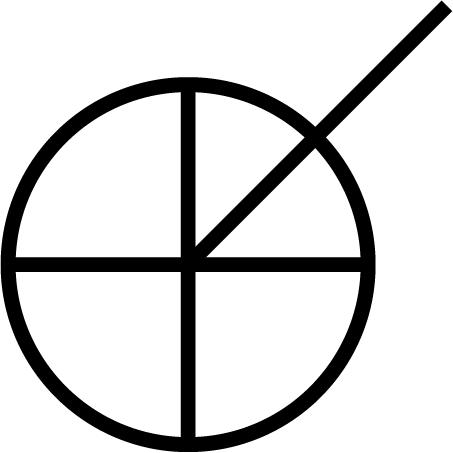
\includegraphics[width=0.8cm]{2.png}
        \end{minipage} &
        \begin{minipage}[t]{\linewidth}
            \vspace{-7pt}
            \begin{itemize}
                \item \textbf{Symbol representing own aircraft}
                \begin{itemize}
                    \item Ground Stabilized: Moves
                    \item Aircraft Stabilized: Stationary
                    \item Outside TID: line drawn from TID center towards symbol
                \end{itemize}
            \end{itemize}
        \end{minipage} \\
        \midrule
        \textbf{TID Cursor} &
        \begin{minipage}[t]{\linewidth}
            \vspace{-7pt}
            \centering
            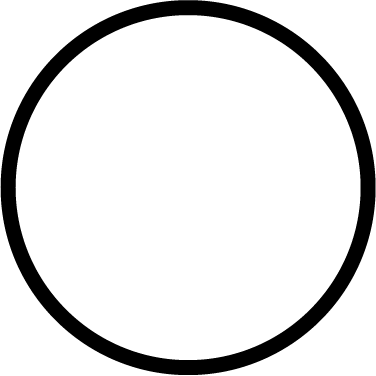
\includegraphics[width=0.8cm]{26.png}
        \end{minipage} &
        \begin{minipage}[t]{\linewidth}
            \vspace{-7pt}
            \begin{itemize}
                \item \textbf{Hook Cursor}
                \begin{itemize}
                    \item Controlled by \textbf{HCU} in \textbf{TID mode}
                \end{itemize}
                \item \textbf{Half-Action}
                \begin{itemize}
                    \item Enables display of symbol
                    \item Enables HCU stick to move cursor
                \end{itemize}
                \item \textbf{Full-Action}
                \begin{itemize}
                    \item Hooks closest symbol
                    \item If no symbol near, cursor dropped at location
                \end{itemize}
            \end{itemize}
        \end{minipage} \\
        \midrule
        \textbf{TWS Steering Centroid} &
        \begin{minipage}[t]{\linewidth}
            \vspace{-7pt}
            \centering
            
\includegraphics[width=0.8cm]{27.png}
        \end{minipage} &
        \begin{minipage}[t]{\linewidth}
            \vspace{-7pt}
            \begin{itemize}
                \item \textbf{Steering centroid of TWS tracks}
                \begin{itemize}
                    \item Selected by WCS for weapons engagement
                \end{itemize}
            \end{itemize}
        \end{minipage} \\
        \midrule
        \multicolumn{2}{c|}{\blue{ONBOARD SENSORS}} & \textbf{Symbol Above Dot} \\
        \midrule
        \textbf{Unknown} &
        \begin{minipage}[t]{\linewidth}
            \vspace{-7pt}
            \centering
            
\includegraphics[width=0.8cm]{3.png}
        \end{minipage} &
        \begin{minipage}[t]{\linewidth}
            \vspace{-7pt}
            \begin{itemize}
                \item \textbf{Unknown Sensor Track}
                \item \textbf{All Returns in RWS}
            \end{itemize}
        \end{minipage} \\
        \midrule
        \textbf{Hostile} &
        \begin{minipage}[t]{\linewidth}
            \vspace{-7pt}
            \centering
            
\includegraphics[width=0.8cm]{4.png}
        \end{minipage} &
        \begin{minipage}[t]{\linewidth}
            \vspace{-7pt}
            \begin{itemize}
                \item \textbf{Sensor Track designated Hostile by RIO}
            \end{itemize}
        \end{minipage} \\
        \midrule
        \textbf{Friend} &
        \begin{minipage}[t]{\linewidth}
            \vspace{-7pt}
            \centering
            
\includegraphics[width=0.8cm]{5.png}
        \end{minipage} &
        \begin{minipage}[t]{\linewidth}
            \vspace{-7pt}
            \begin{itemize}
                \item \textbf{Sensor Track designated Friendly by RIO}
            \end{itemize}
        \end{minipage} \\
        \midrule
        \textbf{Angle-Tracked Radar Target} &
        \begin{minipage}[t]{\linewidth}
            \vspace{-7pt}
            \centering
            
\includegraphics[width=0.55cm]{6.png}
        \end{minipage} &
        \begin{minipage}[t]{\linewidth}
            \vspace{-7pt}
            \begin{itemize}
                \item \textbf{Radar Angle Tracking}
                \begin{itemize}
                    \item Jamming Target
                \end{itemize}
            \end{itemize}
        \end{minipage} \\
        \midrule
        \textbf{Angle-Tracked Radar Target with Altitude Difference Ranging} &
        \begin{minipage}[t]{\linewidth}
            \vspace{-7pt}
            \centering
            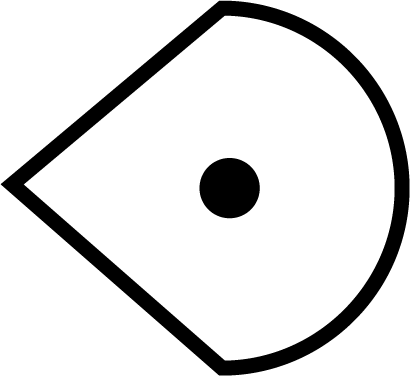
\includegraphics[width=0.8cm]{7.png}
        \end{minipage} &
        \begin{minipage}[t]{\linewidth}
            \vspace{-7pt}
            \begin{itemize}
                \item \textbf{Radar Angle Tracking}
                \begin{itemize}
                    \item Jamming Target
                    \item Alt. diff. ranging
                \end{itemize}
            \end{itemize}
        \end{minipage} \\
        \midrule
        \textbf{TCS-Angle Tracked Target} &
        \begin{minipage}[t]{\linewidth}
            \vspace{-7pt}
            \centering
            
\includegraphics[width=0.55cm]{10.png}
        \end{minipage} &
        \begin{minipage}[t]{\linewidth}
            \vspace{-7pt}
            \begin{itemize}
                \item \textbf{TCS Angle Tracking}
            \end{itemize}
        \end{minipage} \\
        \midrule
        \textbf{TCS-Angle Tracked Target with Altitude Difference Ranging} &
        \begin{minipage}[t]{\linewidth}
            \vspace{-7pt}
            \centering
            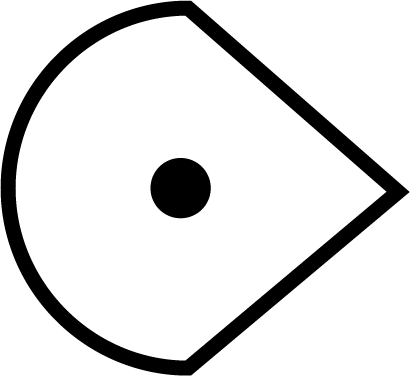
\includegraphics[width=0.8cm]{11.png}
        \end{minipage} &
        \begin{minipage}[t]{\linewidth}
            \vspace{-7pt}
            \begin{itemize}
                \item \textbf{TCS Angle Tracking}
                \begin{itemize}
                    \item Alt. diff. ranging
                \end{itemize}
            \end{itemize}
        \end{minipage} \\
        \midrule
        \multicolumn{2}{c|}{\blue{D/L TARGETS}} & \textbf{Symbol Below Dot} \\
        \midrule
        \textbf{Unknown} &
        \begin{minipage}[t]{\linewidth}
            \vspace{-7pt}
            \centering
            
\includegraphics[width=0.8cm]{12.png}
        \end{minipage} &
        \begin{minipage}[t]{\linewidth}
            \vspace{-7pt}
            \begin{itemize}
                \item \textbf{D/L Track designated Unknown by Source}
            \end{itemize}
        \end{minipage} \\
        \midrule
        \textbf{Hostile} &
        \begin{minipage}[t]{\linewidth}
            \vspace{-7pt}
            \centering
            
\includegraphics[width=0.8cm]{13.png}
        \end{minipage} &
        \begin{minipage}[t]{\linewidth}
            \vspace{-7pt}
            \begin{itemize}
                \item \textbf{D/L Track designated Hostile by Source}
            \end{itemize}
        \end{minipage} \\
        \midrule
        \textbf{Friendly} &
        \begin{minipage}[t]{\linewidth}
            \vspace{-7pt}
            \centering
            
\includegraphics[width=0.8cm]{14.png}
        \end{minipage} &
        \begin{minipage}[t]{\linewidth}
            \vspace{-7pt}
            \begin{itemize}
                \item \textbf{D/L Track designated Friendly by Source}
            \end{itemize}
        \end{minipage} \\
        \midrule
        \multicolumn{2}{c}{\blue{MANUAL REF POINTS}} & \\
        \midrule
        \textbf{Home base} &
        \begin{minipage}[t]{\linewidth}
            \vspace{-7pt}
            \centering
            
\includegraphics[width=0.8cm]{15.png}
        \end{minipage} &
        \begin{minipage}[t]{\linewidth}
            \vspace{-7pt}
            \begin{itemize}
                \item \textbf{Waypoint Representing}
                \begin{itemize}
                    \item Home Base
                    \item Carrier
                    \item Airfield
                \end{itemize}
            \end{itemize}
        \end{minipage} \\
        \midrule
        \textbf{Waypoint} &
        \begin{minipage}[t]{\linewidth}
            \vspace{-7pt}
            \centering
            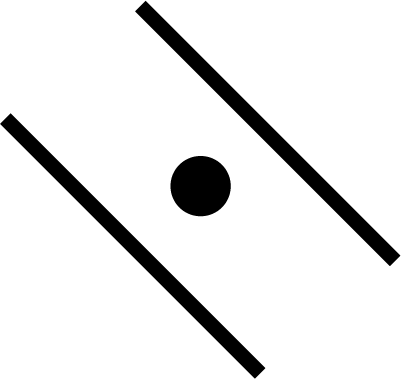
\includegraphics[width=0.8cm]{16.png}
        \end{minipage} &
        \begin{minipage}[t]{\linewidth}
            \vspace{-7pt}
            \begin{itemize}
                \item \textbf{Nav Waypoint}
                \item \textbf{Supplanted by Number}
                \begin{itemize}
                    \item 1, 2, or 3
                \end{itemize}
            \end{itemize}
        \end{minipage} \\
        \midrule
        \textbf{Defended Point} &
        \begin{minipage}[t]{\linewidth}
            \vspace{-7pt}
            \centering
            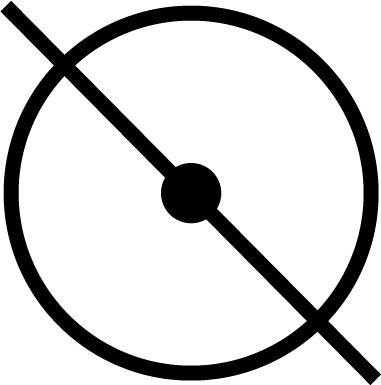
\includegraphics[width=0.8cm]{17.png}
        \end{minipage} &
        \begin{minipage}[t]{\linewidth}
            \vspace{-7pt}
            \begin{itemize}
                \item \textbf{Waypoint to Defend}
            \end{itemize}
        \end{minipage} \\
        \midrule
        \textbf{Fixed Point} &
        \begin{minipage}[t]{\linewidth}
            \vspace{-7pt}
            \centering
            
\includegraphics[width=0.8cm]{18.png}
        \end{minipage} &
        \begin{minipage}[t]{\linewidth}
            \vspace{-7pt}
            \begin{itemize}
                \item \textbf{Generic Waypoint}
            \end{itemize}
        \end{minipage} \\
        \midrule
        \textbf{Hostile Area} &
        \begin{minipage}[t]{\linewidth}
            \vspace{-7pt}
            \centering
            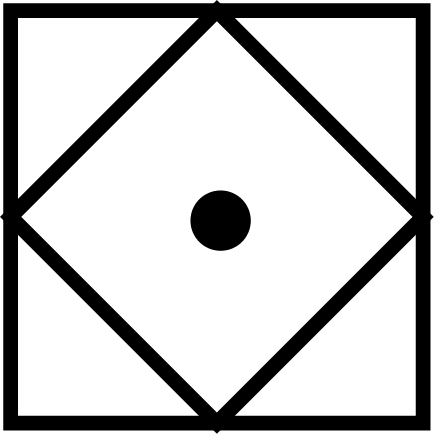
\includegraphics[width=0.8cm]{19.png}
        \end{minipage} &
        \begin{minipage}[t]{\linewidth}
            \vspace{-7pt}
            \begin{itemize}
                \item \textbf{Waypoint Indicating Hostile Area}
            \end{itemize}
        \end{minipage} \\
        \midrule
        \textbf{Surface Target} &
        \begin{minipage}[t]{\linewidth}
            \vspace{-7pt}
            \centering
            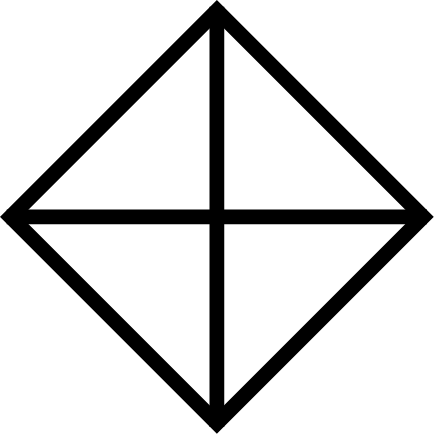
\includegraphics[width=0.8cm]{20.png}
        \end{minipage} &
        \begin{minipage}[t]{\linewidth}
            \vspace{-7pt}
            \begin{itemize}
                \item \textbf{Waypoint Indicating Surface Target}
            \end{itemize}
        \end{minipage} \\
        \midrule
        \textbf{IP} &
        \begin{minipage}[t]{\linewidth}
            \vspace{-7pt}
            \centering
            
\includegraphics[width=0.8cm]{21.png}
        \end{minipage} &
        \begin{minipage}[t]{\linewidth}
            \vspace{-7pt}
            \begin{itemize}
                \item \textbf{Initial Point}
                \begin{itemize}
                    \item Waypoint for A/G engagement
                \end{itemize}
            \end{itemize}
        \end{minipage} \\
        \midrule
        \multicolumn{2}{c}{\blue{D/L REF POINTS}} & \\
        \midrule
        \textbf{Home Base} &
        \begin{minipage}[t]{\linewidth}
            \vspace{-7pt}
            \centering
            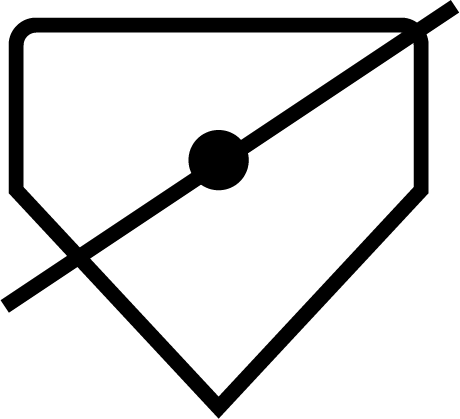
\includegraphics[width=0.8cm]{22.png}
        \end{minipage} &
        \begin{minipage}[t]{\linewidth}
            \vspace{-7pt}
            \begin{itemize}
                \item \textbf{D/L Waypoint Representing Home Base}
            \end{itemize}
        \end{minipage} \\
        \midrule
        \textbf{Waypoint} &
        \begin{minipage}[t]{\linewidth}
            \vspace{-7pt}
            \centering
            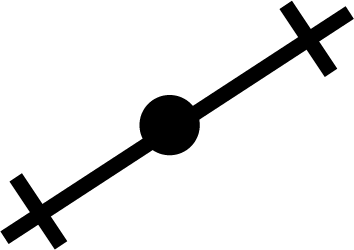
\includegraphics[width=0.8cm]{23.png}
        \end{minipage} &
        \begin{minipage}[t]{\linewidth}
            \vspace{-7pt}
            \begin{itemize}
                \item \textbf{D/L Generic Waypoint}
            \end{itemize}
        \end{minipage} \\
        \midrule
        \textbf{Data Link Fixed Point} &
        \begin{minipage}[t]{\linewidth}
            \vspace{-7pt}
            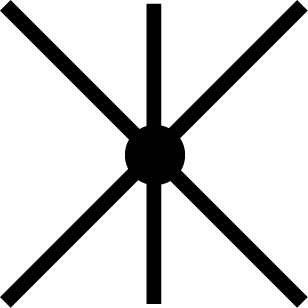
\includegraphics[width=0.8cm]{24.png}
        \end{minipage} &
        \begin{minipage}[t]{\linewidth}
            \vspace{-7pt}
            \begin{itemize}
                \item \textbf{D/L Waypoint Representing Fixed Point}
            \end{itemize}
        \end{minipage} \\
        \midrule
        \textbf{Surface Target} &
        \begin{minipage}[t]{\linewidth}
            \vspace{-7pt}
            \centering
            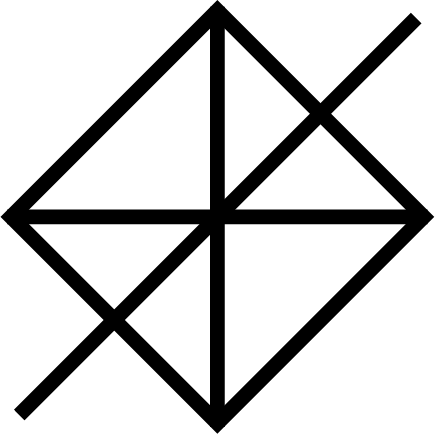
\includegraphics[width=0.8cm]{25.png}
        \end{minipage} &
        \begin{minipage}[t]{\linewidth}
            \vspace{-7pt}
            \begin{itemize}
                \item \textbf{D/L Waypoint Representing a Surface Target}
            \end{itemize}
        \end{minipage} \\
        \midrule
        \multicolumn{2}{c}{\blue{POS SYMB MODIFIERS}} &  \\
        \midrule
        \textbf{Mandatory Attack} &
        \begin{minipage}[t]{\linewidth}
            \vspace{-7pt}
            \centering
            
\includegraphics[width=0.8cm]{28.png}
        \end{minipage} &
        \begin{minipage}[t]{\linewidth}
            \vspace{-7pt}
            \begin{itemize}
                \item \textbf{Additional Symbology on TWS Track}
                \begin{itemize}
                    \item Horizontal bar through center dot
                \end{itemize}
                \item \textbf{Selected by RIO}
                \begin{itemize}
                    \item Only 1 target can be designated
                    \item Guaranteed WCS priority number
                \end{itemize}
            \end{itemize}
        \end{minipage} \\
        \midrule
        \textbf{Data Link Destroy }&
        \begin{minipage}[t]{\linewidth}
            \vspace{-7pt}
            \centering
            
\includegraphics[width=0.8cm]{29.png}
        \end{minipage} &
        \begin{minipage}[t]{\linewidth}
            \vspace{-7pt}
            \begin{itemize}
                \item \textbf{Additional Symbology on D/L Track}
                \begin{itemize}
                    \item Horizontal bar through center dot
                \end{itemize}
                \item \textbf{Selected by Source}
                \begin{itemize}
                    \item No effect on WCS prioritization
                \end{itemize}
            \end{itemize}
        \end{minipage} \\
        \midrule
        \textbf{Do Not Attack} &
        \begin{minipage}[t]{\linewidth}
            \vspace{-7pt}
            \centering
            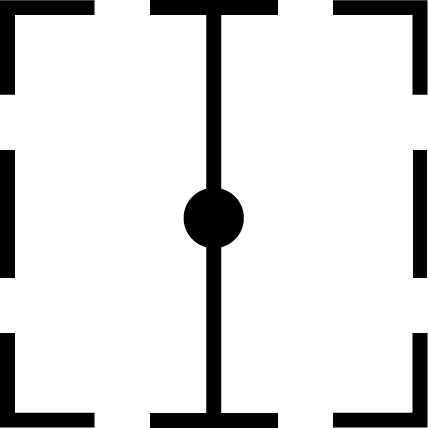
\includegraphics[width=0.8cm]{30.png}
        \end{minipage} &
        \begin{minipage}[t]{\linewidth}
            \vspace{-7pt}
            \begin{itemize}
                \item \textbf{Additional Symbology on TWS or D/L Track}
                \begin{itemize}
                    \item Vertical bar through center dot
                \end{itemize}
                \item \textbf{If Set by RIO}
                \begin{itemize}
                    \item Removes WCS prioritization
                \end{itemize}
            \end{itemize}
        \end{minipage} \\
        \midrule
        \textbf{Multiple Targets} &
        \begin{minipage}[t]{\linewidth}
            \vspace{-7pt}
            \centering
            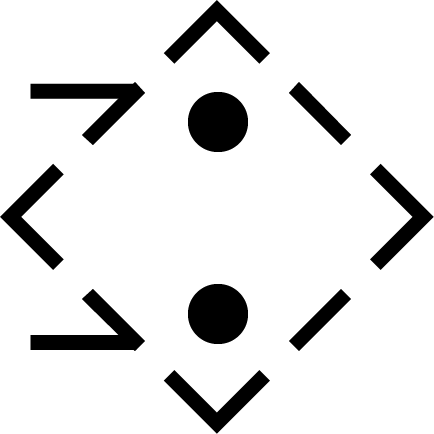
\includegraphics[width=0.8cm]{31.png}
        \end{minipage} &
        \begin{minipage}[t]{\linewidth}
            \vspace{-7pt}
            \begin{itemize}
                \item \textbf{Additional Symbology on TWS or D/L Track}
                \begin{itemize}
                    \item Horizontal bar on left side of symbol
                \end{itemize}
                \item \textbf{Indicates Multiple Targets}
            \end{itemize}
        \end{minipage} \\
        \midrule
        \textbf{Data Link Challenge} &
        \begin{minipage}[t]{\linewidth}
            \vspace{-7pt}
            \centering
            
\includegraphics[width=0.8cm]{32.png}
        \end{minipage} &
        \begin{minipage}[t]{\linewidth}
            \vspace{-7pt}
            \begin{itemize}
                \item \textbf{Additional Symbology on D/L Track}
                \begin{itemize}
                    \item Small \textbf{V} with center at center dot
                \end{itemize}
                \item \textbf{Command to Visually Identify}
            \end{itemize}
        \end{minipage} \\
        \midrule
        \textbf{Track Extrapolated} &
        \begin{minipage}[t]{\linewidth}
            \vspace{-7pt}
            \centering
            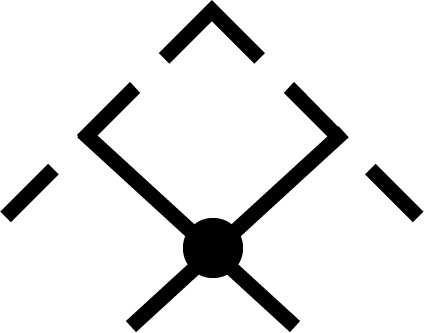
\includegraphics[width=0.8cm]{33.png}
        \end{minipage} &
        \begin{minipage}[t]{\linewidth}
            \vspace{-7pt}
            \begin{itemize}
                \item \textbf{Additional Symbology on TWS or D/L Track}
                \begin{itemize}
                    \item Small \textbf{X} with center at center dot
                \end{itemize}
                \item \textbf{No Update within 8 seconds}
                \begin{itemize}
                    \item Track deleted after 14 seconds
                    \item Or after 2 min if track hold
                \end{itemize}
            \end{itemize}
        \end{minipage} \\
        \midrule
        \textbf{Altitude Numerics} &
        \begin{minipage}[t]{\linewidth}
            \vspace{-7pt}
            \centering
            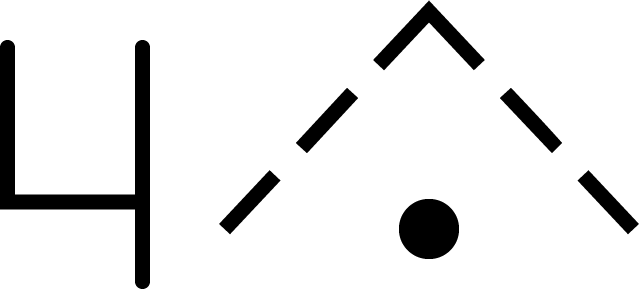
\includegraphics[width=1cm]{34.png}
        \end{minipage} &
        \begin{minipage}[t]{\linewidth}
            \vspace{-7pt}
            \begin{itemize}
                \item \textbf{Altitude to Nearest Ten Thousand}
                \begin{itemize}
                    \item example: 35000-45000
                \end{itemize}
            \end{itemize}
        \end{minipage} \\
        \midrule
        \textbf{Firing Order Numerics} &
        \begin{minipage}[t]{\linewidth}
            \vspace{-7pt}
            \centering
            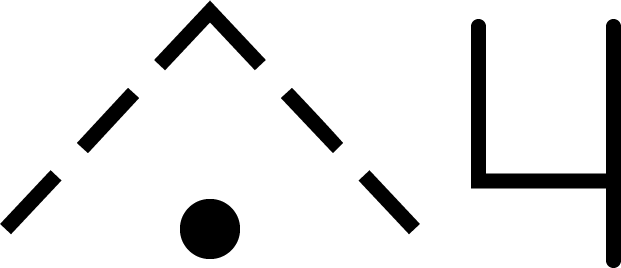
\includegraphics[width=1cm]{35.png}
        \end{minipage} &
        \begin{minipage}[t]{\linewidth}
            \vspace{-7pt}
            \begin{itemize}
                \item \textbf{Indicates AIM-54 Prioritization}
                \begin{itemize}
                    \item Numbers 1-6
                    \item Only in TWS
                \end{itemize}
            \end{itemize}
        \end{minipage} \\
        \midrule
        \textbf{Time-to-Impact (TTI)} &
        \begin{minipage}[t]{\linewidth}
            \vspace{-7pt}
            \centering
            
\includegraphics[width=1cm]{47.png}
        \end{minipage} &
        \begin{minipage}[t]{\linewidth}
            \vspace{-7pt}
            \begin{itemize}
                \item \textbf{After AIM-54 Launch}
                \begin{itemize}
                    \item Prioritization replaced with estimated TTI
                \end{itemize}
                \item \textbf{Flashes after Pitbull}
            \end{itemize}
        \end{minipage} \\
        \midrule
        \textbf{Velocity Vector} &
        \begin{minipage}[t]{\linewidth}
            \vspace{-7pt}
            \centering
            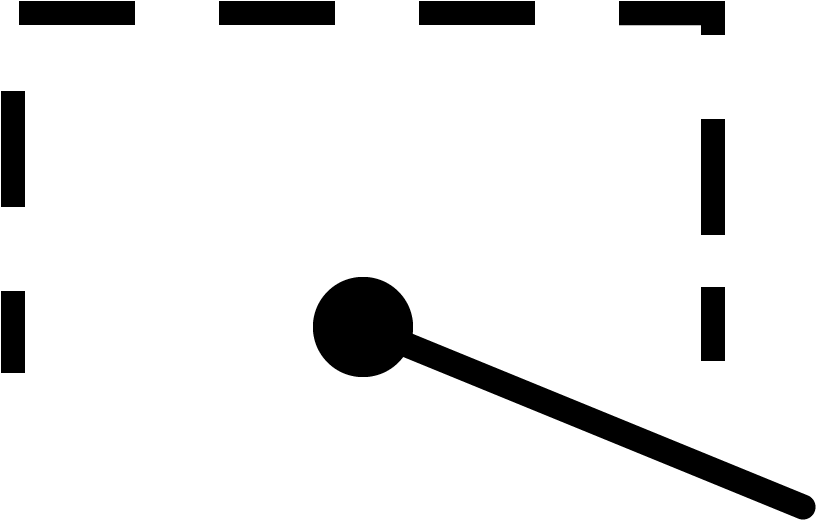
\includegraphics[width=0.8cm]{36.png}
        \end{minipage} &
        \begin{minipage}[t]{\linewidth}
            \vspace{-7pt}
            \begin{itemize}
                \item \textbf{Additional Symbology from center Dot}
                \begin{itemize}
                    \item Direction represents track heading
                    \item Length represents speed
                \end{itemize}
                \item \textbf{Varies with Mode}
                \begin{itemize}
                    \item Ground Stabilized: true heading and ground speed
                    \item Aircraft Stabilized: relative heading and velocity
                \end{itemize}
            \end{itemize}
        \end{minipage} \\
        \midrule
        \textbf{Launch Zone Vectors} &
        \begin{minipage}[t]{\linewidth}
            \vspace{-7pt}
            \centering
            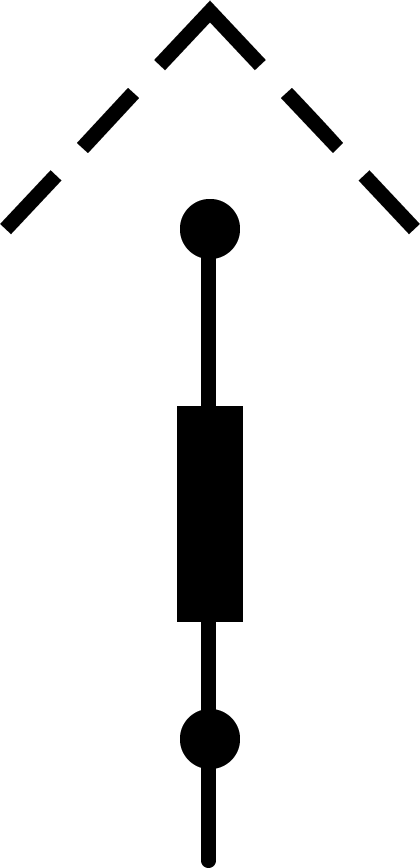
\includegraphics[width=0.8cm]{37.png}
        \end{minipage} &
        \begin{minipage}[t]{\linewidth}
            \vspace{-7pt}
            \centering
            
\includegraphics[width=5cm]{lzv.png}
        \end{minipage}
        \begin{minipage}[t]{\linewidth}
            \begin{itemize}
                \item \textbf{Additional Symbology for AIM-54}
                \begin{itemize}
                    \item Selected manually by RIO
                    \item Or 60 seconds from max launch
                \end{itemize}
                \item \textbf{TUMR}
                \begin{itemize}
                    \item Time-Until-Minimum-Range
                    \item Max: 180 seconds, 1.5 inches
                \end{itemize}
                \item \textbf{TUOR}
                \begin{itemize}
                    \item Time-Until-Optimal-Range
                    \item Start of bar is 8 seconds from optimum
                \end{itemize}
                \item \textbf{TUIR}
                \begin{itemize}
                    \item Time-Until-In-Range
                \end{itemize}
            \end{itemize}
        \end{minipage} \\
        \midrule
        \textbf{Jamming Strobe} &
        \begin{minipage}[t]{\linewidth}
            \vspace{-7pt}
            \centering
            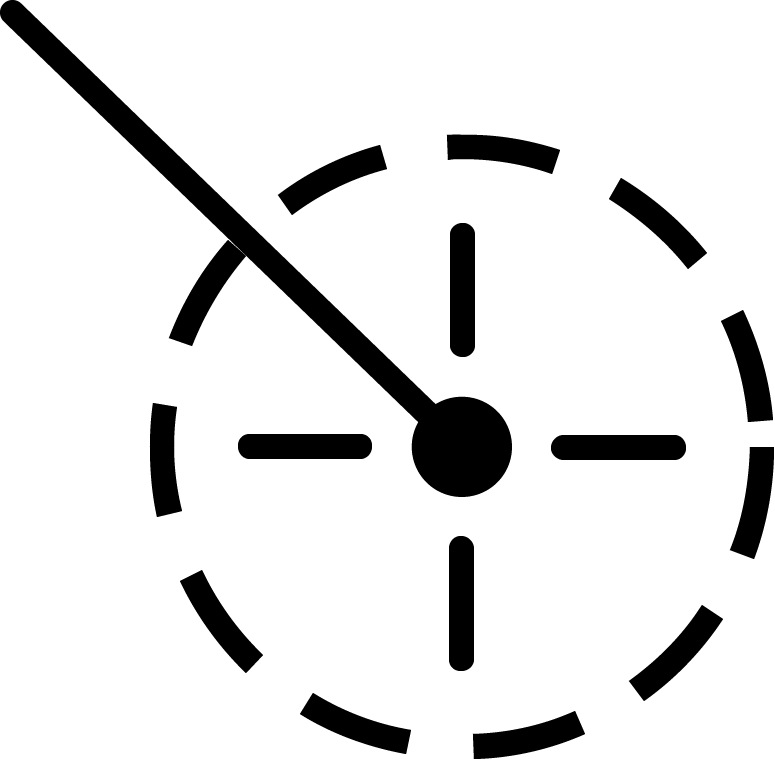
\includegraphics[width=0.8cm]{38.png}
        \end{minipage} &
        \begin{minipage}[t]{\linewidth}
            \vspace{-7pt}
            \begin{itemize}
                \item \textbf{Line from own AC towards Jammer}
            \end{itemize}
        \end{minipage} \\
        \midrule
        \textbf{Radar Antenna Scan Pattern Azimuth Limit}s &
        \begin{minipage}[t]{\linewidth}
            \vspace{-7pt}
            \centering
            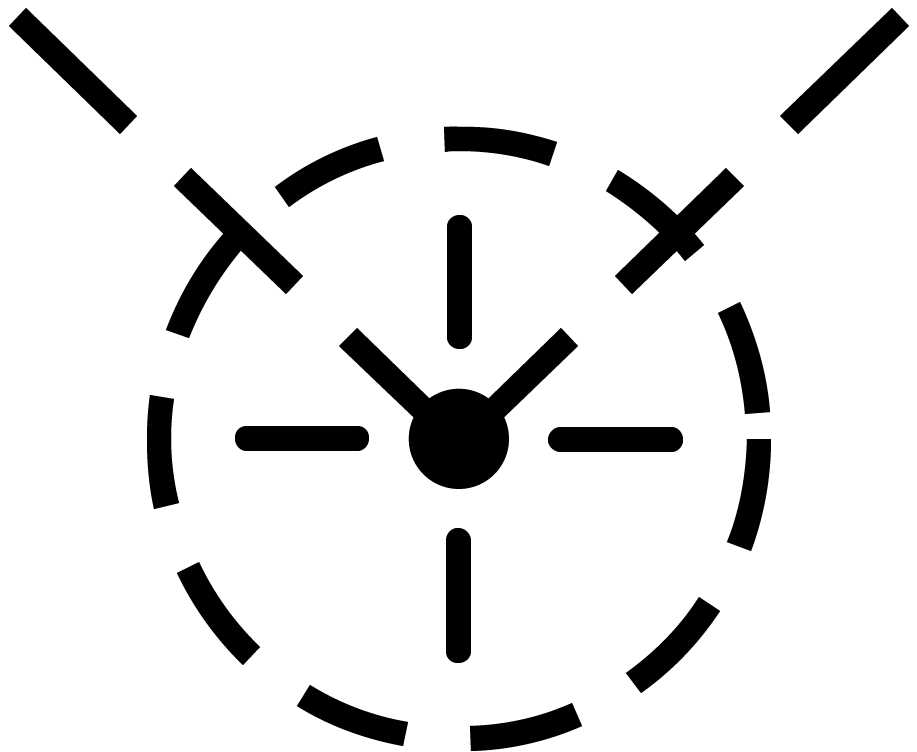
\includegraphics[width=0.8cm]{39.png}
        \end{minipage} &
        \begin{minipage}[t]{\linewidth}
            \vspace{-7pt}
            \begin{itemize}
                \item \textbf{Limits of Current Scan Azimuth}
                \item \textbf{Single Line in STT}
            \end{itemize}
        \end{minipage} \\
        \midrule
        \textbf{Data Link Jamming Strobe} &
        \begin{minipage}[t]{\linewidth}
            \vspace{-7pt}
            \centering
            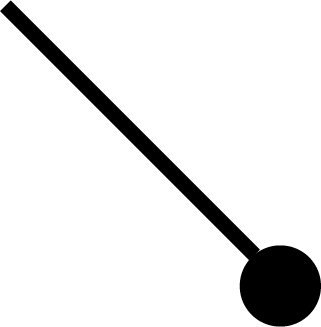
\includegraphics[width=0.8cm]{40.png}
        \end{minipage} &
        \begin{minipage}[t]{\linewidth}
            \vspace{-7pt}
            \begin{itemize}
                \item \textbf{Line from D/L point towards Jammer}
            \end{itemize}
        \end{minipage} \\
        \midrule
        \textbf{Data Link Pointer} &
        \begin{minipage}[t]{\linewidth}
            \vspace{-7pt}
            \centering
            
\includegraphics[width=0.8cm]{41.png}
        \end{minipage} &
        \begin{minipage}[t]{\linewidth}
            \vspace{-7pt}
            \begin{itemize}
                \item \textbf{Additional Symbology on D/L Track}
                \begin{itemize}
                    \item Circle
                    \item Indicates operator concern
                \end{itemize}
            \end{itemize}
        \end{minipage} \\
        \midrule
        \textbf{Data Link Priority Kill} &
        \begin{minipage}[t]{\linewidth}
            \vspace{-7pt}
            \centering
            
\includegraphics[width=0.8cm]{42.png}
        \end{minipage} &
        \begin{minipage}[t]{\linewidth}
            \vspace{-7pt}
            \begin{itemize}
                \item \textbf{Additional Symbology on D/L Track}
                \begin{itemize}
                    \item Square
                    \item Indicates target must be destroyed
                    \item No effect on WCS prioritization
                \end{itemize}
            \end{itemize}
        \end{minipage} \\
        \midrule
        \multicolumn{2}{c}{\blue{ATTACK DISPLAY SYMBOLOGY}} & \\
        \midrule
        \textbf{Artificial Horizon} &
        \begin{minipage}[t]{\linewidth}
            \vspace{-7pt}
            \centering
            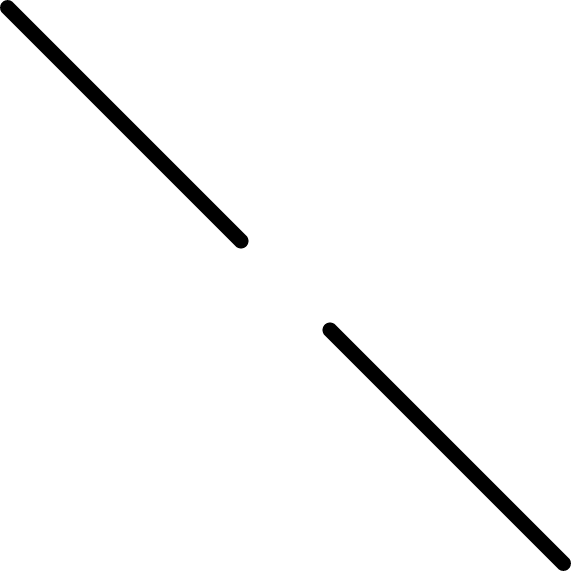
\includegraphics[width=0.8cm]{43.png}
        \end{minipage} &
        \begin{minipage}[t]{\linewidth}
            \vspace{-7pt}
            \begin{itemize}
                \item \textbf{Represents Pitch and Roll}
            \end{itemize}
        \end{minipage} \\
        \midrule
        \textbf{Steering Guidance Symbol} &
        \begin{minipage}[t]{\linewidth}
            \vspace{-7pt}
            \centering
            
\includegraphics[width=0.8cm]{44.png}
        \end{minipage} &
        \begin{minipage}[t]{\linewidth}
            \vspace{-7pt}
            \begin{itemize}
                \item \textbf{Represents Steering Error}
                \begin{itemize}
                    \item Should be placed as near as possible to center of ASE circle
                \end{itemize}
            \end{itemize}
        \end{minipage} \\
        \midrule
        \textbf{Allowable Steering Error Circle} &
        \begin{minipage}[t]{\linewidth}
            \vspace{-7pt}
            \centering
            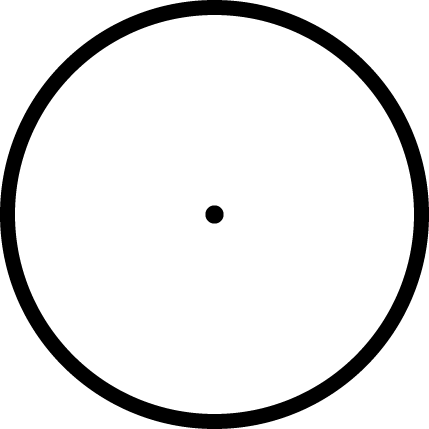
\includegraphics[width=0.8cm]{45.png}
        \end{minipage} &
        \begin{minipage}[t]{\linewidth}
            \vspace{-7pt}
            \begin{itemize}
                \item \textbf{Indicates Allowable Steering Error for Missile Launch}
                \item \textbf{Size Varies with Geometry, Mode, Missile}
            \end{itemize}
        \end{minipage} \\
        \midrule
        \textbf{Breakaway Indication} &
        \begin{minipage}[t]{\linewidth}
            \vspace{-7pt}
            \centering
            
\includegraphics[width=0.8cm]{27.png}
        \end{minipage} &
        \begin{minipage}[t]{\linewidth}
            \vspace{-7pt}
            \begin{itemize}
                \item \textbf{Appears when Target Range Less than Minimum for Selected Weapon}
            \end{itemize}
        \end{minipage} \\
        \bottomrule
    \end{longtable}
\end{center}

\clearpage

\section{INDICATORS}

\subsection{THREAT ADVISORY INDICATORS}
\begin{center}
    \begin{tabular}{p{1.5cm} | p{8.5cm}}
        \toprule
        \blue{Light} & \blue{Description} \\
        \midrule
        \textbf{IFF} & Friendly IFF signal received but no reply generated \\
        \midrule
        \textbf{RCV} & ALQ-126 DECM is receiving a signal \\
        \midrule
        \textbf{XMIT} & ALQ-126 DECM is transmitting \\
        \midrule
        \textbf{SAM} & \textbf{Steady} -- Lockon from SAM detected \\
        & \textbf{Flashing} -- SAM launch detected \\
        \midrule
        \textbf{AAA} & \textbf{Steady} -- Lockon from AAA detected \\
        & \textbf{Flashing} -- AAA engagement detected \\
        \midrule
        \textbf{CW} & CW emitter detected \\
        \midrule
        \textbf{AI} & Airborne Intercepter lockon detected \\
        \bottomrule
    \end{tabular}
\end{center}

\subsection{INS STATUS INDICATORS}
\begin{center}
    \begin{tabular}{p{1.5cm} p{1.5cm} | p{8cm}}
        \toprule
        \blue{STBY} & \blue{READY} & \blue{Description} \\
        \midrule
        \textbf{ON} & \textbf{ON} &
        \begin{minipage}[t]{\linewidth}
            \vspace{-7pt}
            \begin{itemize}
                \item Normal during align initialization
                \item Else indicates IMU, NAV COMP, NPS or AHRS Failure
            \end{itemize}
        \end{minipage} \\
        \midrule
        \textbf{ON} & \textbf{OFF} &
        \begin{minipage}[t]{\linewidth}
            \vspace{-7pt}
            \begin{itemize}
                \item Normal during align after initialization
                \item Normal when \textbf{IMU/AM} selected prior to completion of coarse align
            \end{itemize}
        \end{minipage} \\
        \midrule
        \textbf{FLASH} & \textbf{FLASH} &
        \begin{minipage}[t]{\linewidth}
            \vspace{-7pt}
            \begin{itemize}
                \item Alignment not initiated due to suspended alignment (check parking brake)
            \end{itemize}
        \end{minipage} \\
        \midrule
        \textbf{FLASH} & \textbf{OFF} &
        \begin{minipage}[t]{\linewidth}
            \vspace{-7pt}
            \begin{itemize}
                \item Align suspended (check parking brake)
            \end{itemize}
        \end{minipage} \\
        \midrule
        \textbf{OFF} & \textbf{ON} &
        \begin{minipage}[t]{\linewidth}
            \vspace{-7pt}
            \begin{itemize}
                \item Min weapon launch requirements met
            \end{itemize}
        \end{minipage} \\
        \midrule
        \textbf{OFF} & \textbf{OFF} &
        \begin{minipage}[t]{\linewidth}
            \vspace{-7pt}
            \begin{itemize}
                \item System operating normally
            \end{itemize}
        \end{minipage} \\
        \midrule
        \textbf{OFF} & \textbf{FLASH} & (after 5s both off)
        \begin{minipage}[t]{\linewidth}
            \vspace{-7pt}
            \begin{itemize}
                \item Occurs when \textbf{IMU/AM} selected and IMU is aligned. If another mode not selected within 5 s, alignment lost, INS not available
            \end{itemize}
        \end{minipage} \\
        \midrule
        \textbf{OFF} & \textbf{FLASH} & 
        \begin{minipage}[t]{\linewidth}
            \vspace{-7pt}
            \begin{itemize}
                \item Alignment suspended past mission alert criteria with parking brake off
            \end{itemize}
        \end{minipage} \\
        \bottomrule
    \end{tabular}
\end{center}

\clearpage

\subsection{VDI CAUTION INDICATORS}
\begin{center}
    \begin{tabular}{p{2.8cm} | p{9cm}}
        \toprule
        \blue{Light} & \blue{Description} \\
        \midrule
        \textbf{ADJ A/C} & Indicates other aircraft close to own traffic pattern \\
        \midrule
        \textbf{LANDING CHK} & Indicates carrier has channel ready for ACL, crew should prepare for carrier landing, center needles \\
        \midrule
        \textbf{ACL READY} & Indicates CATCC has aquired aircraft and is transmitting glidepath information \\
        \midrule
        \textbf{A/P CPLR} & Indicates CATCC is ready to control aircraft \\
        \midrule
        \textbf{CMD CONTROL} & Indicates aircraft is under data link control for landing \\
        \midrule
        \textbf{10 SECONDS} & Indicates that carrier motion is added to data link info and commands during landing \\
        & Indicates 10 seconds to arrival at the next point in approach pattern in other modes \\
        \midrule
        \textbf{TILT} & Caution that data link command received for the last 2 seconds during ACL \\
        & When not in ACL it indicates no data link messages during last 10 seconds \\
        \midrule
        \textbf{VOICE} & Caution that CATCC not ready for ACL, switch to standard voice procedures \\
        \midrule
        \textbf{AUTO THRO} & Caution that autothrottle has been disengaged \\
        \midrule
        \textbf{A/P REF} & Indicates autopilot selected but not engaged. Exception altitude and heading hold \\
        \midrule
        \textbf{WAVEOFF} & Indicates waveoff commanded \\
        \midrule
        \textbf{WING SWEEP} & Caution indicating failure in both wing-sweep channels or disengagement of spider detent \\
        \midrule
        \textbf{REDUCE SPEED} & Indicates flap retraction failure with greater than 225 knots indicated airspeed \\
        & Also indicates safe Mach number exceeded \\
        \midrule
        \textbf{ALT LOW} & Non functional, refer to radar altimeter \\
        \bottomrule
    \end{tabular}
\end{center}

%fills rest of page with blanks
\cleardoublepage